\section{Wall-resolved mesh requirements}
\label{sec:evaluation:mesh-families-yplus}

Wall-resolved RANS meshes are commonly designed to place the first cell centre at \(y_1^+\le1\). The NASA Turbulence Modeling Resource describes this as conventional practice for simulations that integrate the turbulence model to the wall.\footnote{\url{https://tmbwg.github.io/turbmodels/flatplate_val_ypluseffect.html}} A general basis for treating this rule as sufficient for hypersonic cold-wall heat-flux convergence was not identified in the literature reviewed here. Fletcher~\cite[p.~401]{fletcher2012computational}, for example, recommends \(y^+<5\) to resolve the near-wall velocity profile and notes that compressible temperature profiles may require \(y^+<2\). These recommendations motivate placing the first point within the viscous sublayer, but do not establish a convergence criterion for heat-transfer under hypersonic cold-wall conditions.
\par\medskip

The first-cell centre lies at \(y_1=\delta_n=\Delta y_1/2\) for the
wall-normal cells used here, where \(\Delta y_1\) is the full first-cell
thickness. Its distance in wall units is \(y_1^+=\rho_w u_\tau y_1/\mu_w\),
with friction velocity \(u_\tau=\sqrt{|\tau_w|/\rho_w}\).
The alternative resolution indicator is the first-cell acoustic Reynolds number
\begin{equation}
    Re_{\mathrm{cell1}}=\frac{\rho_w a_w\,\delta_n}{\mu_w}.
    \label{eq:evaluation:first-cell-acoustic-re}
\end{equation}
Here \(\rho_w\), \(a_w\) and \(\mu_w\) are the density, speed of sound and
dynamic viscosity evaluated at the wall.

Dilley~\cite{dilley2001evaluation} found that a cell Reynolds number of approximately unity was required for grid-converged hypersonic heating predictions with the Baldwin--Lomax model. His definition uses first-cell properties and the full cell height, so its numerical threshold cannot be transferred directly to Equation~\eqref{eq:evaluation:first-cell-acoustic-re}, but it gives an indication. Related criteria have also been used for laminar stagnation-point heating~\cite{papadopoulos1999current}, aeroheating calculations for the X-38~\cite{loomis2004aeroheating} and mesh adaptation in LAURA~\cite{Thompson2024LAURA}.
\par\medskip

Figures~\ref{fig:evaluation:SA-mesh-convergence-behaviour} and~\ref{fig:evaluation:SST-mesh-convergence-behaviour} illustrate the effect of reducing the first-cell height for M6Tw025. They show the streamwise development of the skin-friction coefficient \(C_f\) and Stanton number \(C_h\), expressed in terms of \(Re_\tau\), at fixed downstream spacing. For SA, the curves nearly coincide from \(y_1^+=1.24\) down to the finest mesh. The \(k\)--\(\omega\) SST model requires refinement to approximately \(y_1^+=0.129\) before mesh convergence is reached. The weaker first-cell sensitivity of SA is qualitatively consistent with the NASA flat-plate study cited above, which reports greater sensitivity for models using an \(\omega\) equation.

\begin{figure}[H]
    \centering
    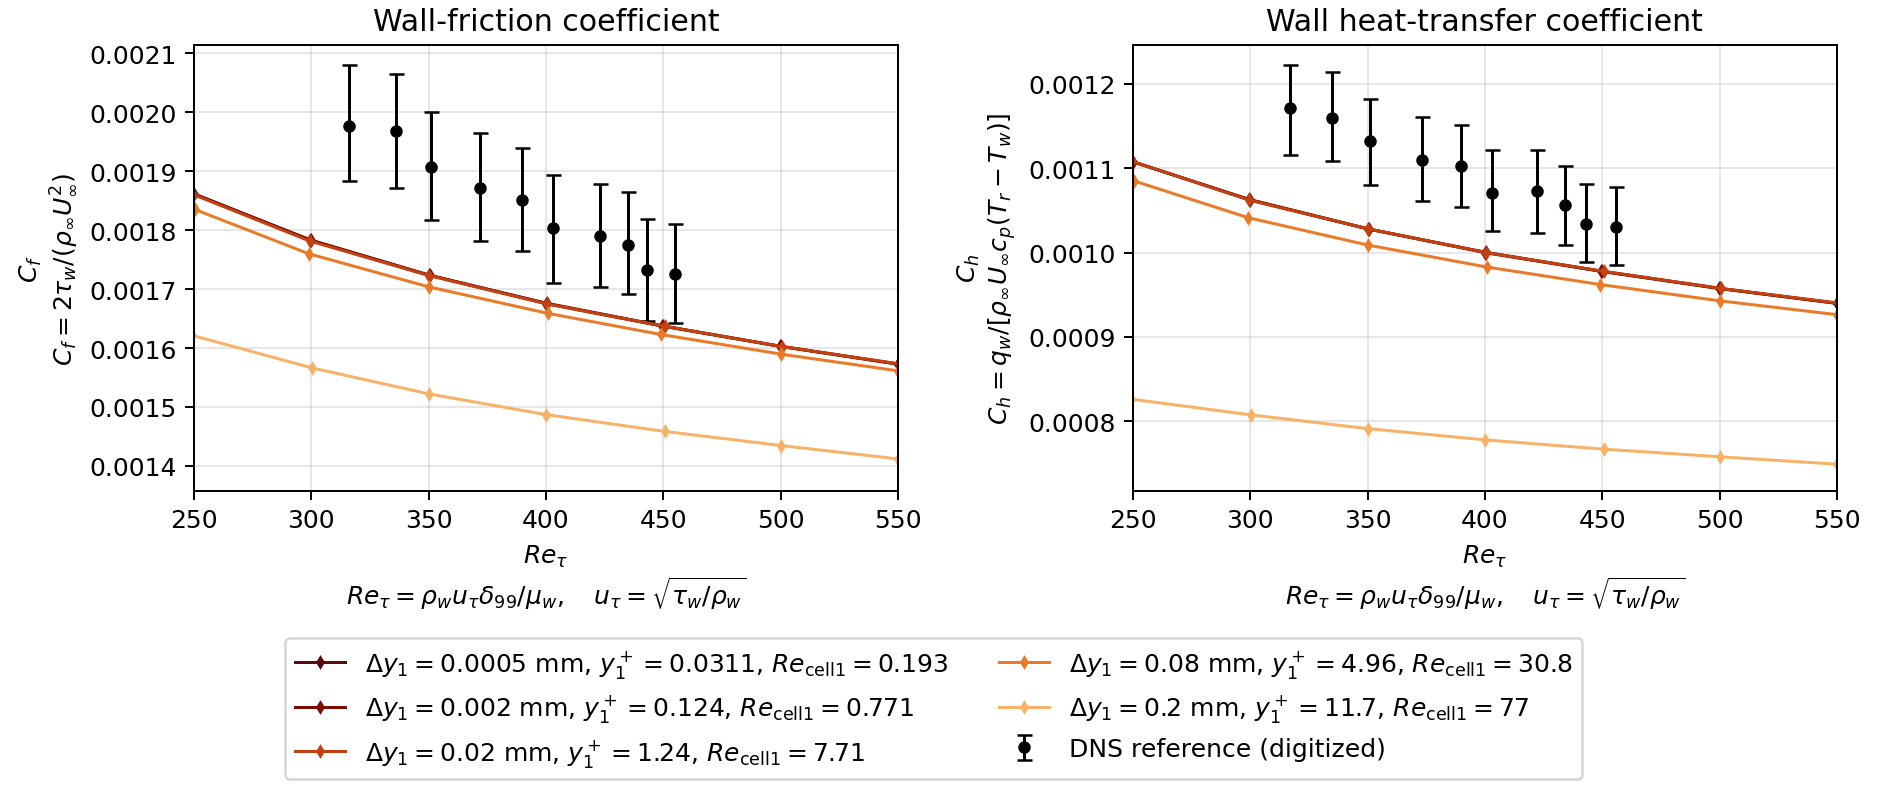
\includegraphics[width=\linewidth]{06_Eval_Methodology/06_Figures/SA_wall_coefficients_vs_dns.png}
    \caption[M6Tw025: first-cell mesh sensitivity with SA]{First-cell mesh sensitivity of the SA predictions for M6Tw025: skin-friction coefficient \(C_f\) (left) and Stanton number \(C_h\) (right) versus \(Re_\tau\), with fixed downstream spacing \(\Delta x=5\,\mathrm{mm}\). Coloured curves show the different first-cell thicknesses \(\Delta y_1\); black symbols denote the digitized DNS reference~\cite{zhang2018direct}. The \(y_1^+\) values reported in the legend are evaluated at each mesh's DNS-matched station, defined by \(Re_{\delta2}=1135\), rather than representing a constant value along the plate.}
    \label{fig:evaluation:SA-mesh-convergence-behaviour}
\end{figure}

\begin{figure}[H]
    \centering
    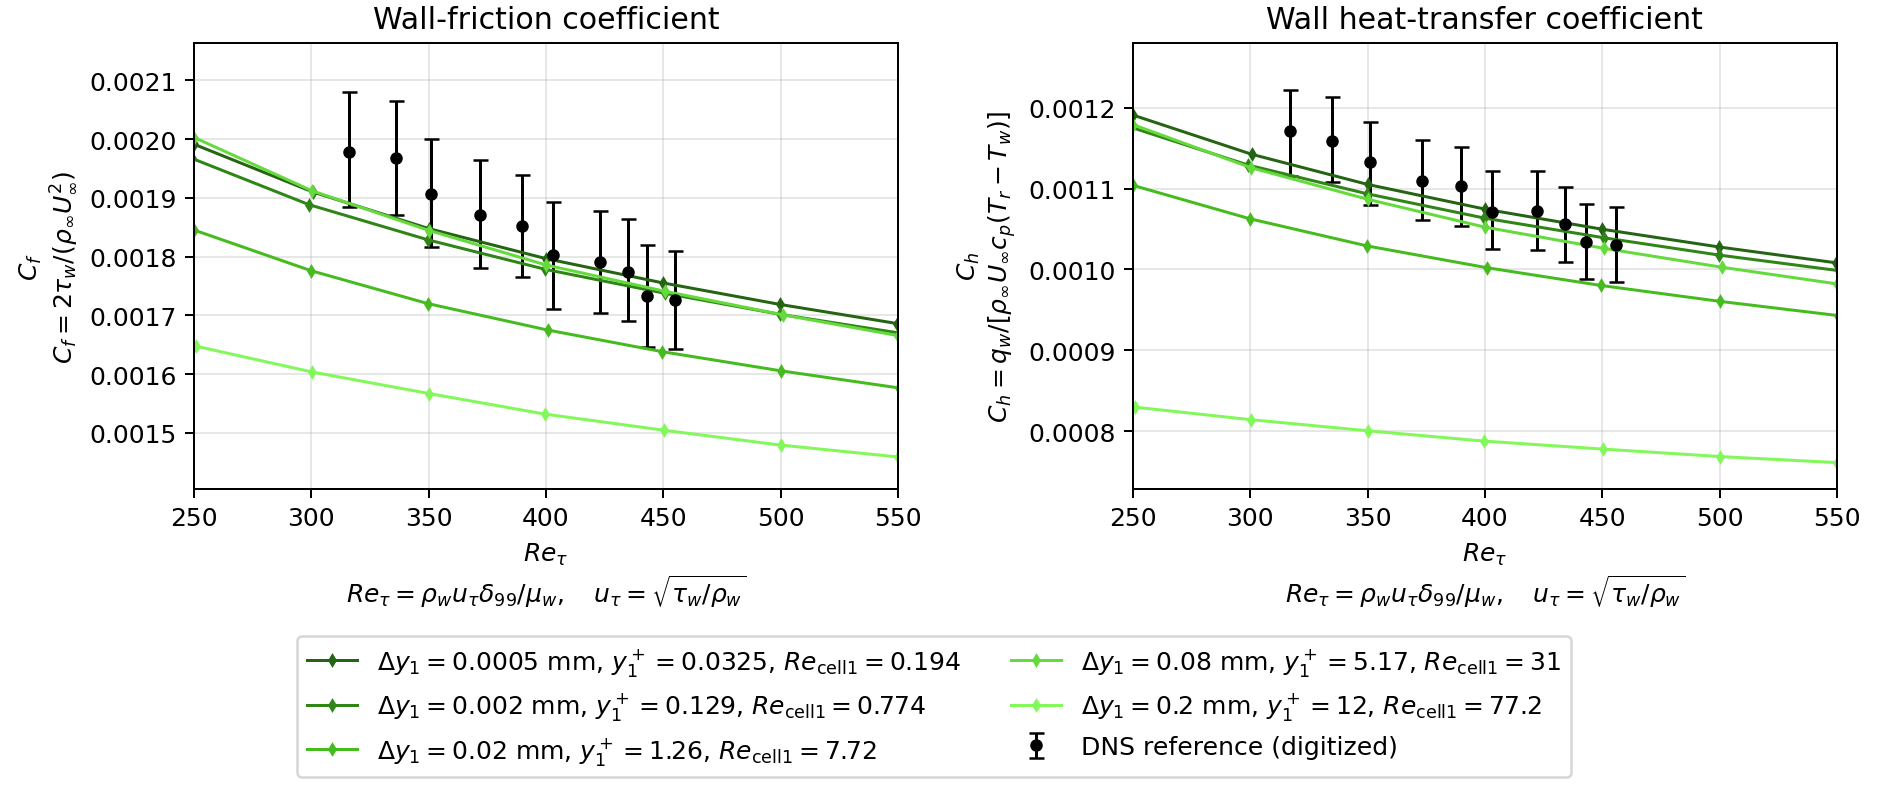
\includegraphics[width=\linewidth]{06_Eval_Methodology/06_Figures/kwSST_wall_coefficients_vs_dns.png}
    \caption[M6Tw025: first-cell mesh sensitivity with SST]{First-cell mesh sensitivity of the \(k\)--\(\omega\) SST predictions for M6Tw025: skin-friction coefficient \(C_f\) (left) and Stanton number \(C_h\) (right) versus \(Re_\tau\), with fixed downstream spacing \(\Delta x=5\,\mathrm{mm}\). Coloured curves show the different first-cell thicknesses \(\Delta y_1\); black symbols denote the digitized DNS reference~\cite{zhang2018direct}. The \(y_1^+\) values reported in the legend are evaluated at each mesh's DNS-matched station, defined by \(Re_{\delta2}=1135\), rather than representing a constant value along the plate.}
    \label{fig:evaluation:SST-mesh-convergence-behaviour}
\end{figure}

Appendix~\ref{app:zpg:mesh-convergence} extends the wall-normal refinement study to all twelve ZPG flat-plate cases. Streamwise-refinement tests for M6Tw025 showed negligible sensitivity of heat-flux and skin-friction to the downstream spacing when the leading edge was refined. The remaining mesh studies therefore focus on the wall-normal direction. They report skin-friction and, for the isothermal cases, heat-transfer against \(y_1^+\) and \(Re_{\mathrm{cell1}}\) at the DNS-matched downstream stations. For the investigated hypersonic cold-wall cases, these results support \(Re_{\mathrm{cell1}}\le1\) as a practical resolution guideline, particularly for SST, in preference to relying on \(y_1^+\le1\) alone.
\par\medskip

The wall-gradient approximation provides a plausible explanation for this stringent resolution requirement. As discussed in Section~\ref{sec:openFOAM_qw_tauw}, OpenFOAM/HiSA evaluates the wall gradients from the difference between the wall value and the first off-wall cell value. Accurate wall fluxes therefore require this secant to approximate the local wall derivative. Placing the first cell within the nominal viscous sublayer is insufficient if the velocity or temperature gradient varies appreciably across that distance. The cold-wall profile shapes in Figures~\ref{fig:background:dns-velocity-profiles} and~\ref{fig:background:dns-temperature-profiles} motivate this distinction between resolving a profile and resolving its wall slope. The mesh studies establish the numerical basis for the wall-resolved model comparisons in Section~\ref{sec:comparative:zpg:wall-resolved-baselines}, where agreement with the DNS reference is assessed separately there.
